\section{Durchführung}
\label{sec:Durchführung}
\begin{figure}[H]
    \centering
    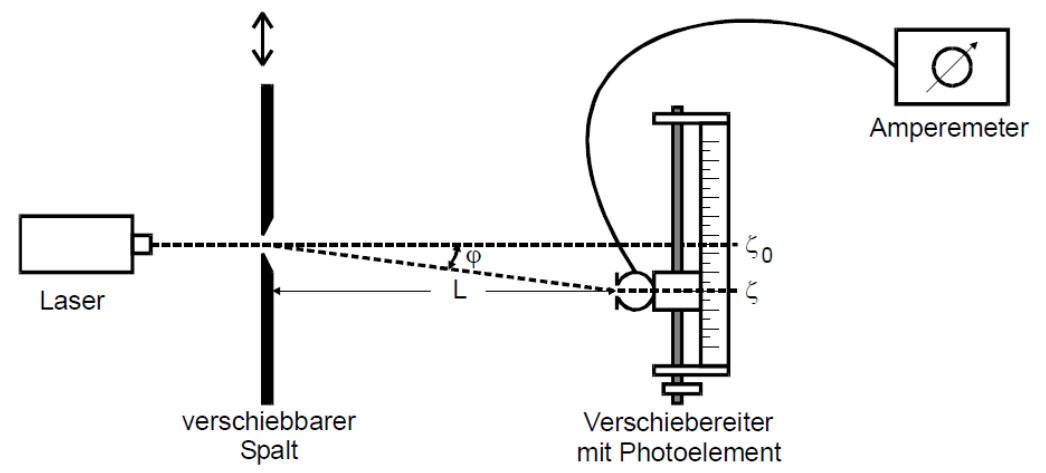
\includegraphics{Versuchsaufbau.png}
    \caption{Versuchsaufbau \cite{V406}.}
    \label{fig:d}
\end{figure}
Für den Versuch wird der Versuchsaufbau wie in Abbildung \ref{fig:d} dargestellt, aufgebaut. 
Allerdings wird kein verschiebbarer Spalt benutzt, sondern Spalt-Schablonen.
Als erstes wird der Dunkelstrom gemessen, dafür wird das Ampermeter auf plus gestellt. 
Nachdem dies gemacht wurde, wird das Amperemeter wieder auf minus gestell und ein Einfachspalt eingehängt, dann wird mit Hilfe des Ampermeters das Maximum gesucht. 
Vom Ort des Maximums wird die Messaperatur je um einen Millimeter verschoben bis zum Ende der Skala bei 5cm. 
Nach jedem Verstellen wird der Wert auf dem Ampermeter notiert. Danach wird wieder vom Maximum aus in ein Millimeter schritten 
verstellt, allerdings in die andere Richtung bis zum Ende der Skala bei 0cm. Es werden wieder pro Schritt die Messwerte notiert.
Anschließend wird ein Doppelspalt eingehangen und die Prozedur wie beim Einfachspalt durchgeführt.
